\documentclass{ctexart}
\usepackage{graphicx}
\usepackage{amsmath}
\usepackage{amsthm}
\usepackage{amssymb}
\usepackage{fancyhdr}
\usepackage{ifthen}
\usepackage{syntonly}
\usepackage[colorlinks, CJKbookmarks=true, linkcolor=red]{hyperref}
\pagestyle{plain}
\usepackage[raggedright]{titlesec}
\newtheorem{性质}{性质}
\newtheorem{定理}{定理}
\newtheorem{推论}{推论}
\begin{document}
\title{作业}
\author{计算机科学与技术系52班 杨定澄 \and 学号:2015011274 \and E-mail:892431401@qq.com}
\date{}
\maketitle
\section*{第一题}
\subsection*{(1)}
原本的式子是$P(error|x)=\min(P(\omega_1|x),P(\omega_2|x))$,现改为$2P(\omega_1|x)P(\omega_2|x)$。

设$P(\omega_1|x)=t,t \in [0,1]$,由于$P(\omega_1|x)+P(\omega_2|x)=1$,故$P(\omega_2|x)=1-t$。

$\therefore 2P(\omega_1|x)P(\omega_2|x)=2t(1-t),\min(P(\omega_1|x),P(\omega_2|x))=\min(t,1-t)$

当$0.5 \le t \le 1$时,$2t \ge 1,2t(1-t) \ge 1 \times (1-t)=1-t=\min(t,1-t)$。

当$0 \le t <0.5$时,$2(1-t) \ge 1,2t(1-t) \ge 1 \times t=t=\min(t,1-t)$

综上所述,$2P(\omega_|x)P(\omega_2|x) \ge P(error|x)$

\[\therefore \int_{-\infty}^{\infty}2P(\omega_1|x)P(\omega_2|x)P(x)dx \ge \int_{-\infty}^{\infty}\min(P(\omega_1|x),P(\omega_2|x))P(x)dx\]

\subsection*{(2)}
不妨令$\forall x,P(\omega_1|x)=P(\omega_2|x)=\frac{1}{2}$,那么按照原来的式子计算

\[P(error)=\int_{-\infty}^{\infty}\min(P(\omega_1|x),P(\omega_2|x))P(x)dx=\int_{-\infty}^{\infty}\frac{1}{2}P(x)dx=\frac{1}{2}\int_{-\infty}^{\infty}P(x)dx=\frac{1}{2}\]

按照新式子计算的话

\[P(error)=\int_{-\infty}^{\infty}\alpha P(\omega_1|x)P(\omega_2|x)P(x)dx=\int_{-\infty}^{\infty}\frac{\alpha}{4}P(x)dx=\frac{\alpha}{4}\int_{-\infty}^{\infty}P(x)dx=\frac{\alpha}{4}\]

因为$\alpha<2$,故$\frac{\alpha}{4}<\frac{1}{2}$,故这种算法无法得到误差上界。
\subsection*{(3)}
类似$(1)$问,设$P(\omega_1|x)=t,t \in [0,1]$,由于$P(\omega_1|x)+P(\omega_2|x)=1$,故$P(\omega_2|x)=1-t$。

由于$t \in [0,1]$,故$0 \le t \le 1,0 \le 1-t \le 1$,从而得出$t(1-t) \le t,t(1-t) \le 1-t$,即$t(1-t) \le \min(t,1-t)$

\[\therefore \int_{-\infty}^{\infty}P(\omega_1|x)P(\omega_2|x)P(x)dx \le \int_{-\infty}^{\infty}\min(P(\omega_1|x),P(\omega_2|x))P(x)dx\]

\subsection*{(4)}
不妨令$\forall x,P(\omega_1|x)=\frac{1+\frac{1}{\beta}}{2},P(\omega_2|x)=1-P(\omega_1|x)$。

这样的话,$\frac{1}{\beta}<P(\omega_1|x)<1,\beta P(\omega_1|x)>\beta\frac{1}{\beta}=1$,故$\beta P(\omega_1|x)P(\omega_2|x)>P(\omega_2|x)\ge \min(P(\omega_1|x),P(\omega_2|x))$

\[\therefore \int_{-\infty}^{\infty}\beta P(\omega_1|x)P(\omega_2|x)P(x)dx > \int_{-\infty}^{\infty}\min(P(\omega_1|x),P(\omega_2|x))P(x)dx\]

因此这种算法无法得到误差下界。
\section*{第二题}
\subsection*{(1)}
如果我们作出$P(\omega_i|x)$的图像,就会得到三条折线,那么最优决策点$x_1^*,x_2^*$必然是折线的交点。

但是折线的交点有很多种情况:

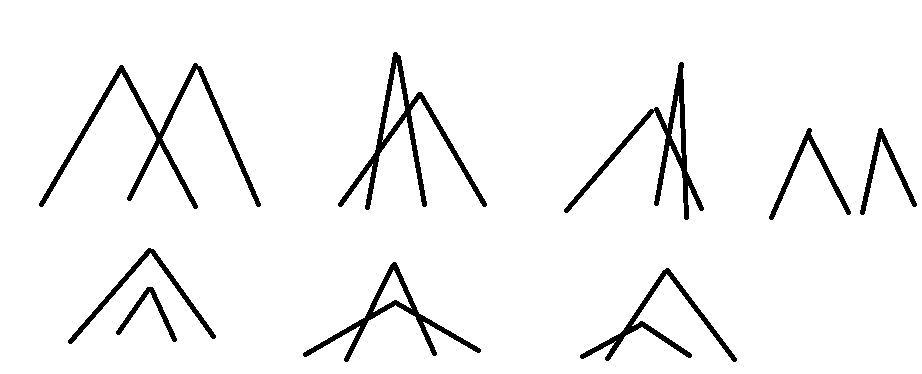
\includegraphics[width=5in]{1.png}

如上图,这么多种情况会给我们的讨论带来极大的麻烦,他们有的甚至会导致最优决策点不止两个。

为了方便起见,我们希望所有的情况都是形如第一种的。为此,我们给$\delta$增加一些约束条件,让函数的分布曲线唯一:

\begin{align}
\mu_1-\delta_1<\mu_1<\mu_2-\delta_2<\mu_1+\delta_1<\mu_2<\mu_3-\delta_3<\mu_2+\delta_2<\mu_3<\mu_3+\delta_3
\end{align}


与之对应的,函数图像将长这样:

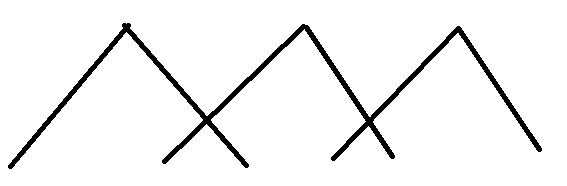
\includegraphics[width=5in]{2.png}。

这是一种比较简单的情形,我们只用求出$\omega_1$右半部分折线与$\omega_2$左半部分折线的交点和$\omega_2$右半部分折线与$\omega_3$左半部分折线的交点即可。

根据$x_1^*,x_2^*$的定义,此时显然有$\mu_2-\delta_2 \le x_1^* \le \mu_1+\delta_1,\mu_3-\delta_3 \le x_2^* \le \mu_2+\delta_2$。

$P(\omega_i|x)=P(x|\omega_i)P(\omega_i)=T(\mu_i,\delta_i)P(\omega_i)=\frac{(\delta_i-|x-\mu_i|)}{\delta_i^2}P(\omega_i)$

故

\[\begin{cases}
\frac{\delta_1-x_1^*+\mu_1}{\delta_1^2}P(\omega_1)=\frac{\delta_2-\mu_2+x_1^*}{\delta_2^2}P(\omega_2) \\
\frac{\delta_2-x_2^*+\mu_2}{\delta_2^2}P(\omega_2)=\frac{\delta_3-\mu_3+x_2^*}{\delta_3^2}P(\omega_3)
\end{cases}\]

解得
\[\begin{cases}
x_1^*=[\frac{\delta_1+\mu_1}{\delta_1^2}P(\omega_1)-\frac{\delta_2-\mu_2}{\delta_2^2}P(\omega_2)]/[\frac{P(\omega_1)}{\delta_1^2}+\frac{P(\omega_2}{\delta_2^2}] \\
x_2^*=[\frac{\delta_2+\mu_2}{\delta_2^2}P(\omega_2)-\frac{\delta_3-\mu_3}{\delta_3^2}P(\omega_3)]/[\frac{P(\omega_2)}{\delta_2^2}+\frac{P(\omega_3}{\delta_3^2}]
\end{cases}\]
\subsection*{(2)}
\begin{align*}
R=&\int_{R_1}[\lambda_{11}P(\omega_1)P(x|\omega_1)+\lambda_{12}P(\omega_2)P(x|\omega_2)+\lambda_{13}P(\omega_3)P(x|\omega_3)]dx\\
 +&\int_{R_2}[\lambda_{21}P(\omega_1)P(x|\omega_1)+\lambda_{22}P(\omega_2)P(x|\omega_2)+\lambda_{23}P(\omega_3)P(x|\omega_3)]dx\\
 +&\int_{R_3}[\lambda_{31}P(\omega_1)P(x|\omega_1)+\lambda_{32}P(\omega_2)P(x|\omega_2)+\lambda_{33}P(\omega_3)P(x|\omega_3)]dx\\
 =&P(\omega_1)[\lambda_{11}\int_{R_1}P(x|\omega_1)dx+\lambda_{21}\int_{R_2}P(x|\omega_1)dx+\lambda_{31}\int_{R_3}P(x|\omega_1)dx]\\
 +&P(\omega_2)[\lambda_{12}\int_{R_1}P(x|\omega_2)dx+\lambda_{22}\int_{R_2}P(x|\omega_2)dx+\lambda_{32}\int_{R_3}P(x|\omega_2)dx]\\
 +&(1-P(\omega_1)-P(\omega_2)[\lambda_{13}\int_{R_1}P(x|\omega_3)dx+\lambda_{23}\int_{R_2}P(x|\omega_3)dx+\lambda_{33}\int_{R_3}P(x|\omega_3)dx]\\
 =&P(\omega_1)A+P(\omega_2)B+C
\end{align*}

其中:
\begin{align*}
A=&[\lambda_{11}\int_{R_1}P(x|\omega_1)dx+\lambda_{21}\int_{R_2}P(x|\omega_1)dx+\lambda_{31}\int_{R_3}P(x|\omega_1)dx]\\
 -&[\lambda_{13}\int_{R_1}P(x|\omega_3)dx+\lambda_{23}\int_{R_2}P(x|\omega_3)dx+\lambda_{33}\int_{R_3}P(x|\omega_3)dx]\\
B=&[\lambda_{12}\int_{R_1}P(x|\omega_2)dx+\lambda_{22}\int_{R_2}P(x|\omega_2)dx+\lambda_{32}\int_{R_3}P(x|\omega_2)dx]\\
 -&[\lambda_{13}\int_{R_1}P(x|\omega_3)dx+\lambda_{23}\int_{R_2}P(x|\omega_3)dx+\lambda_{33}\int_{R_3}P(x|\omega_3)dx]\\
C=&[\lambda_{13}\int_{R_1}P(x|\omega_3)dx+\lambda_{23}\int_{R_2}P(x|\omega_3)dx+\lambda_{33}\int_{R_3}P(x|\omega_3)dx]
\end{align*}

不妨设$S_{ij}=\int_{R_i}P(x|\omega_j)dx$,那么有
\begin{align*}
A=&[\lambda_{11}S_{11}+\lambda_{21}S_{21}+\lambda_{31}S_{31}]-[\lambda_{13}S_{13}+\lambda_{23}S_{23}+\lambda_{33}S_{33}]\\
B=&[\lambda_{12}S_{12}+\lambda_{22}S_{22}+\lambda_{32}S_{32}]-[\lambda_{13}S_{13}+\lambda_{23}S_{23}+\lambda_{33}S_{33}]\\
C=&[\lambda_{13}S_{13}+\lambda_{23}S_{23}+\lambda_{33}S_{33}]
\end{align*}

我们仍然采用$(1)$式的条件,来计算$S_{ij}$,从图中可以看出,$\mu_2-\delta_2 \le x_1^* \le \mu_1+\delta_1,\mu_3-\delta_3 \le x_2^* \le \mu_2+\delta_2$
\[
\begin{cases}
&S_{21}=\int_{R_2}P(x|\omega_1)dx=\int_{x_1^*}^{\mu_1+\delta_1}\frac{\delta_1-x+\mu_1}{\delta_1^2}dx=\frac{(\mu_1+\delta_1-x_1^*)^2}{2\delta_1^2}\\
&S_{31}=0\\
&S_{11}=1-S_{21}-S_{31}=1-\frac{(\mu_1+\delta_1-x_1^*)^2}{2\delta_1^2}\\
&S_{23}=\int_{R_2}P(x|\omega_3)dx=\int_{\mu_3-\delta_3}^{x_2^*}\frac{\delta_3-\mu_3+x}{\delta_3^2}dx=\frac{(x_2^*-\mu_3+\delta_3)^2}{2\delta_3^2}\\
&S_{13}=0\\
&S_{33}=1-S_{23}-S_{13}=1-\frac{(x_2^*-\mu_3+\delta_3)^2}{2\delta_3^2}\\
&S_{12}=\int_{R_1}P(x|\omega_2)dx=\int_{\mu_2-\delta_2}^{x_1^*}\frac{\delta_2-x+\mu_2}{\delta_2^2}dx=\frac{(x_1^*-\mu_2+\delta_2)^2}{2\delta_2^2}\\
&S_{32}=\int_{R_3}P(x|\omega_2)dx=\int_{x_2^*}^{\mu_2+\delta_2}\frac{\delta_2-x+\mu_2}{\delta_2^2}dx=\frac{(\mu_2+\delta_2-x_2^*)^2}{2\delta_2^2}\\
&S_{22}=1-S_{12}-S_{32}=1-\frac{(x_1^*-\mu_2+\delta_2)^2}{2\delta_2^2}-\frac{(\mu_2+\delta_2-x_2^*)^2}{2\delta_2^2}
\end{cases}
\]

由于要求的是极小化极大决策,故这里满足
\[
\lambda_{ij}=
\begin{cases}
1 & i=j \\
0 & i \neq j
\end{cases}
\]

代入后有方程组
\[\begin{cases}
&\frac{\mu_1+\delta_1-x_1^*}{\delta_1}=\frac{x_2^*-\mu_3+\delta_3}{\delta_3}\\
&\frac{(x_1^*-\mu_2+\delta_2)^2+(\mu_2+\delta_2-x_2^*)^2}{\delta_2^2}=\frac{(x_2^*-\mu_3+\delta_3)^2}{\delta_3^2}
\end{cases}\]

解此二元方程组即可。

联立可解得$x_1^*,x_2^*$。
\subsection*{(3)}
三个折线的定义域区间分别是$[-1,1],[0,1],[0,2]$,根据$x_1^*,x_2^*$的定义显然有$0 \le x_1^* \le x_2^* \le 1$,可以由此计算$S_{i1}$和$S_{i3}$

\[
\begin{cases}
&S_{21}=\int_{x_1^*}^{x_2^*}\frac{1-(x-0)}{1^2}dx=\frac{(x_2^*-x_1^*)(2-x_1^*-x_2^*)}{2}\\
&S_{31}=\int_{x_2^*}^1\frac{1-(x-0)}{1^2}dx=\frac{(1-x_2^*)^2}{2}\\
&S_{11}=1-S_{21}-S_{31}=1-\frac{(x_1^*-1)^2}{2}\\
&S_{13}=\int_0^{x_1^*}\frac{1-(1-x_1^*)}{1^2}dx=\frac{(x_1^*)^2}{2}\\
&S_{23}=\int_{x_1^*}^{x_2^*}\frac{1-(1-x)}{1^2}dx=\frac{(x_2^*)^2-(x_1^*)^2}{2}\\
&S_{33}=1-S_{13}-S_{23}=1-\frac{(x_2^*)^2}{2}
\end{cases}
\]
为求极小化极大决策,取
\[
\lambda_{ij}=
\begin{cases}
1 & i=j \\
0 & i \neq j
\end{cases}
\]

由于$S_{21}+S_{31}-S_{13}-S_{23}=0$,故$(x_1^*)^2-(x_2^*)^2-2x_1^*+1=0$,解得$(x_1^*-1)^2=(x_2^*)^2$

考虑到$0 \le x_1^* \le x_2^* \le 1$,故有$0 \le x_1^* \le 0.5 \le x_2^* \le 1,\textrm{且} x_1^*+x_2^*=1$。

从而可以推出
\[
\begin{cases}
&S_{12}=\int_0^{x_1^*}\frac{0.5-(0.5-x)}{0.5^2}dx=2(x_1^*)^2\\
&S_{32}=\int_{x_2^*}^1\frac{0.5-(x-0.5)}{0.5^2}dx=2(1-x_2^*)^2\\
&S_{22}=1-S_{12}-S_{32}=1-2(x_1^*)^2-2(x_2^*-1)^2
\end{cases}
\]

由于$S_{12}+S_{32}-S_{13}-S_{23}=0,x_2^*=1-x_1^*,0 \le x_1^* \le 0.5$,解得
\[
\begin{cases}
& x_1^*=\frac{-2+4\sqrt{2}}{14} \\
& x_2^*=\frac{16-4\sqrt{2}}{14}
\end{cases}
\]
\subsection*{(4)}
极小化极大风险为$[\lambda_{13}S_{13}+\lambda_{23}S_{23}+\lambda_{33}S_{33}]=S_{13}+S_{23}=\frac{(x_1^*)^2}{2}+\frac{(x_2^*)^2-(x_1^*)^2}{2}=\frac{(x_2^*)^2}{2}$。

由于$x_2^*=\frac{16-4\sqrt{2}}{14}$,故极小化极大风险为$0.2729$。
\end{document}
